\documentclass[11pt,letterpaper]{article}

\usepackage[spanish,es-nodecimaldot]{babel}
\usepackage[no-math]{fontspec}
\setmainfont{EB Garamond}[
  UprightFont    = * Medium,
  ItalicFont     = * Medium Italic,
  BoldFont       = * SemiBold,
  BoldItalicFont = * SemiBold Italic
]

\usepackage{amsmath,amssymb}      % Standard AMS math packages
\usepackage{newtxmath}
\usepackage[bb=libus,bbscaled=1.0]{mathalpha}
\DeclareSymbolFont{operators}{OT1}{ntxtlf}{m}{n}
\SetSymbolFont{operators}{bold}{OT1}{ntxtlf}{b}{n}
\usepackage{microtype}
\microtypesetup{protrusion=false}
\usepackage{mathtools,bm}
\usepackage{enumitem}
\usepackage{geometry}
\usepackage{graphicx}
\usepackage{caption}
\usepackage{xcolor}
\usepackage[most]{tcolorbox}
\usepackage{fancyhdr}
\usepackage{lastpage}
\usepackage[round]{natbib}
\usepackage{xurl}
\usepackage[hidelinks]{hyperref}

\geometry{margin=1in}
\captionsetup[figure]{font=scriptsize,justification=centering}
\definecolor{resultgreen}{HTML}{3F5F4A}
\definecolor{resultback}{HTML}{F7F5EF}

\pagestyle{fancy}
\fancyhf{}
\chead{\small LAT4092 Temas Selectos 3}
\lhead{\small ID: 175199}
\rhead{\small \thepage}
\renewcommand{\headrulewidth}{0pt}


\setlength{\parindent}{0pt}
\setlength{\parskip}{0.68em}
\setlength{\emergencystretch}{3em}
\Urlmuskip=0mu plus 1mu

\newcommand{\E}{\mathbb{E}}
\newcommand{\Prob}{\mathbb{P}}
\newcommand{\Q}{\mathbb{Q}}
\newcommand{\Var}{\operatorname{Var}}
\newcommand{\dd}{\,\mathrm{d}}
\newcommand{\Normal}{\mathcal{N}}
\newcommand{\PhiN}{\Phi}
\newcommand{\pos}[1]{\left(#1\right)^+}

\definecolor{resultblue}{HTML}{23395B}
\definecolor{resultback}{HTML}{FAFAF7}
\definecolor{oldgold}{HTML}{B89B5E}      % dorado editorial discreto

\NewDocumentCommand{\resultbox}{+m}{%
\begin{center}
\begin{tcolorbox}[
    enhanced,
    width=0.92\linewidth,
    colback=resultback,
    colframe=resultback,
    boxrule=0pt,
    arc=5pt,
    outer arc=5pt,
    left=15pt,
    right=14pt,
    top=4pt,
    bottom=12pt,
    boxsep=0pt,
    before skip=10pt,
    after skip=10pt,
    borderline west={4pt}{0.4pt}{resultblue},
    borderline west={0.45pt}{4.2pt}{oldgold},borderline west={0.45pt}{0pt}{oldgold},
    before upper={%
        \setlength{\abovedisplayskip}{5pt}%
        \setlength{\belowdisplayskip}{1pt}%
        \setlength{\abovedisplayshortskip}{3pt}%
        \setlength{\belowdisplayshortskip}{3pt}%
    }
]
#1
\end{tcolorbox}
\end{center}
}
\begin{document}

\begin{center}
{\Large\bfseries Valuación de opciones asiáticas de venta}\par
\vspace{0.25em}
{\large\bfseries Promedio geométrico, promedio aritmético y comparación con opción vanilla}
\end{center}

\begin{abstract}
Se desarrolla un caso de estudio para valuar una opción de venta asiática de promedio geométrico con vencimiento de tres meses y compararla con una put asiática de promedio aritmético y una put europea vanilla. La valuación se realiza bajo un modelo lognormal con costo de acarreo constante. Para el promedio geométrico se emplea la fórmula cerrada de \citet{kemna1990}; para el promedio aritmético se utiliza la aproximación de \citet{turnbull1991}, en la versión presentada por \citet{hull2018}, basada en igualación de los dos primeros momentos. Con los parámetros considerados, las primas son: \(P_{\mathrm{arit}}=4.6415\), \(P_{\mathrm{geom}}=4.6922\) y \(P_{\mathrm{vanilla}}=5.2186\). Por tanto,
\[
P_{\mathrm{arit}}<P_{\mathrm{geom}}<P_{\mathrm{vanilla}}.
\]
\end{abstract}


\section{Introducción}
En los mercados financieros, las opciones asiáticas aparecen de manera natural cuando el riesgo económico de una empresa depende de un precio promedio durante un periodo, y no de un precio específico observado en una sola fecha. Esto ocurre con frecuencia en materias primas, energía, divisas y tasas de interés, donde los contratos comerciales, presupuestos o flujos de efectivo suelen estar ligados a precios promedio mensuales o trimestrales. Por esta razón, las opciones asiáticas son instrumentos útiles para cubrir riesgos de mercado sin concentrar toda la cobertura en el precio de un único día.

En empresas como Pemex, sus ingresos por venta de crudo están expuestos al precio internacional del petróleo, pero su planeación financiera depende del comportamiento promedio del precio durante el periodo en que se realizan ventas, compras, ajustes presupuestales o programas de cobertura, no depende solamente del precio al cierre de un trimestre. De hecho, Pemex reporta el uso de instrumentos financieros derivados, incluyendo opciones de crudo clasificadas como instrumentos de cobertura en su información financiera de 2024 ante la Securities and Exchange Commission \citep{pemex2024sec}.

Pemex muestra que el resultado contable de los derivados puede ser positivo o negativo, según el movimiento de los precios y las condiciones de los contratos. En sus estados financieros dictaminados de 2025, Pemex reportó un rendimiento neto por instrumentos financieros derivados de \(21{,}587{,}903\) miles de pesos en 2025, frente a un costo neto de \(27{,}594{,}230\) miles de pesos en 2024; para opciones de crudo, reportó \(2{,}288{,}069\) miles de pesos en 2025 y \(-898{,}527\) miles de pesos en 2024 \citep{pemex2025estados}. No es que la cobertura sea favorable o desfavorable por sí misma, ya que su función es transformar el perfil de riesgo. Si una empresa quisiera protegerse contra una caída sostenida en el precio promedio del petróleo, una put asiática podría ser más representativa que una put vanilla, porque su pago dependería del promedio observado y no únicamente del precio final. Este tipo de derivado reduce la posibilidad de que un movimiento extremo en una sola fecha determine toda la compensación de la cobertura.

Una vez notada la importancia de este tipo de instrumentos, este trabajo analiza la valuación de opciones asiáticas de venta con tipo de promedio geométrico y aritmético. El promedio geométrico permite obtener una fórmula cerrada, mientras que el promedio aritmético requiere una aproximación por momentos. Finalmente, los resultados se comparan con la prima de una opción vanilla europea con los mismos parámetros.

% Para fijar la notación, se definen las siguientes variables:

% \begin{description}[style=nextline,leftmargin=2.7cm,labelwidth=2.2cm,labelsep=0.45cm,font=\normalfont\itshape]
% \item[\(S_t\):] Precio del activo subyacente al tiempo \(t\).

% \item[\(K\):] Precio de ejercicio. En una put, el pago aumenta cuando el precio promedio relevante queda por debajo de \(K\). 

% \item[\(T\):] Plazo a vencimiento expresado en años.

% \item[\(r\):] Tasa libre de riesgo anual con capitalización continua. Es la tasa de descuento del valor esperado neutral al riesgo.

% \item[\(b\):] Costo de acarreo anual. En modelos con dividendos, usualmente \(b=r-q\); en divisas, \(b=r-r_f\). Aquí se usa directamente el dato \(b=8\%\).

% \item[\(\sigma\):] Volatilidad anual del subyacente. 

% \item[\(A_T\):] Promedio aritmético continuo del subyacente:
% \[
% A_T=\frac{1}{T}\int_0^T S_u\dd u.
% \]

% \item[\(G_T\):] Promedio geométrico continuo del subyacente:
% \[
% G_T=\exp\left(\frac{1}{T}\int_0^T\ln S_u\dd u\right).
% \]

% \item[\(\PhiN(x)\):] Función de distribución acumulada de una normal estándar, \(Z\sim\Normal(0,1)\). 

% \item[\(M_1,M_2\):] Primer y segundo momento del promedio aritmético continuo. La aproximación de \citet{turnbull1991} utiliza estos momentos para aproximar el promedio aritmético mediante una variable lognormal equivalente.

% \item[\(P_A,P_G,P_V\):] Primas de la put asiática aritmética, la put asiática geométrica y la put vanilla, respectivamente.
% \end{description}



\section{Naturaleza financiera de una opción asiática}

Una opción asiática es un derivado dependiente de la trayectoria, porque su pago no se determina únicamente por el precio final del subyacente \(S_T\), sino por algún promedio de los precios observados durante la vida del contrato. Esta característica la distingue de una opción europea vanilla, cuyo pago depende solamente del valor del subyacente en la fecha de vencimiento.

Conviene separar dos clasificaciones. La primera corresponde al sentido del derecho: una opción puede ser call, si otorga exposición alcista, o put, si otorga protección frente a caídas del subyacente. La segunda corresponde a la forma en que interviene el promedio. Una opción asiática puede ser de \emph{average price}, cuando el promedio sustituye al precio del subyacente dentro del pago, o de \emph{average strike}, cuando el promedio sustituye al precio de ejercicio. En este trabajo se consideran puts asiáticas de tipo \emph{average price}. Por tanto, el pago al vencimiento tiene la forma
\begin{equation}
\max\{K-\bar S_T,0\},
\end{equation}
donde \(K\) es el precio de ejercicio y \(\bar S_T\) representa el promedio relevante del subyacente durante el periodo. En particular, \(\bar S_T\) puede ser el promedio aritmético \(A_T\) o el promedio geométrico \(G_T\).

La Figura~\ref{fig:asian-put-oil-path} muestra un ejemplo de una put asiática sobre petróleo. La trayectoria simulada cae durante el periodo y el precio promedio observado queda por debajo del precio de ejercicio; por ello, la put asiática genera una compensación positiva igual a \(K-A_T\). Además, se muestra el promedio geométrico \(G_T\), que es menor que el promedio aritmético \(A_T\). 

\begin{figure}[htbp]
\centering
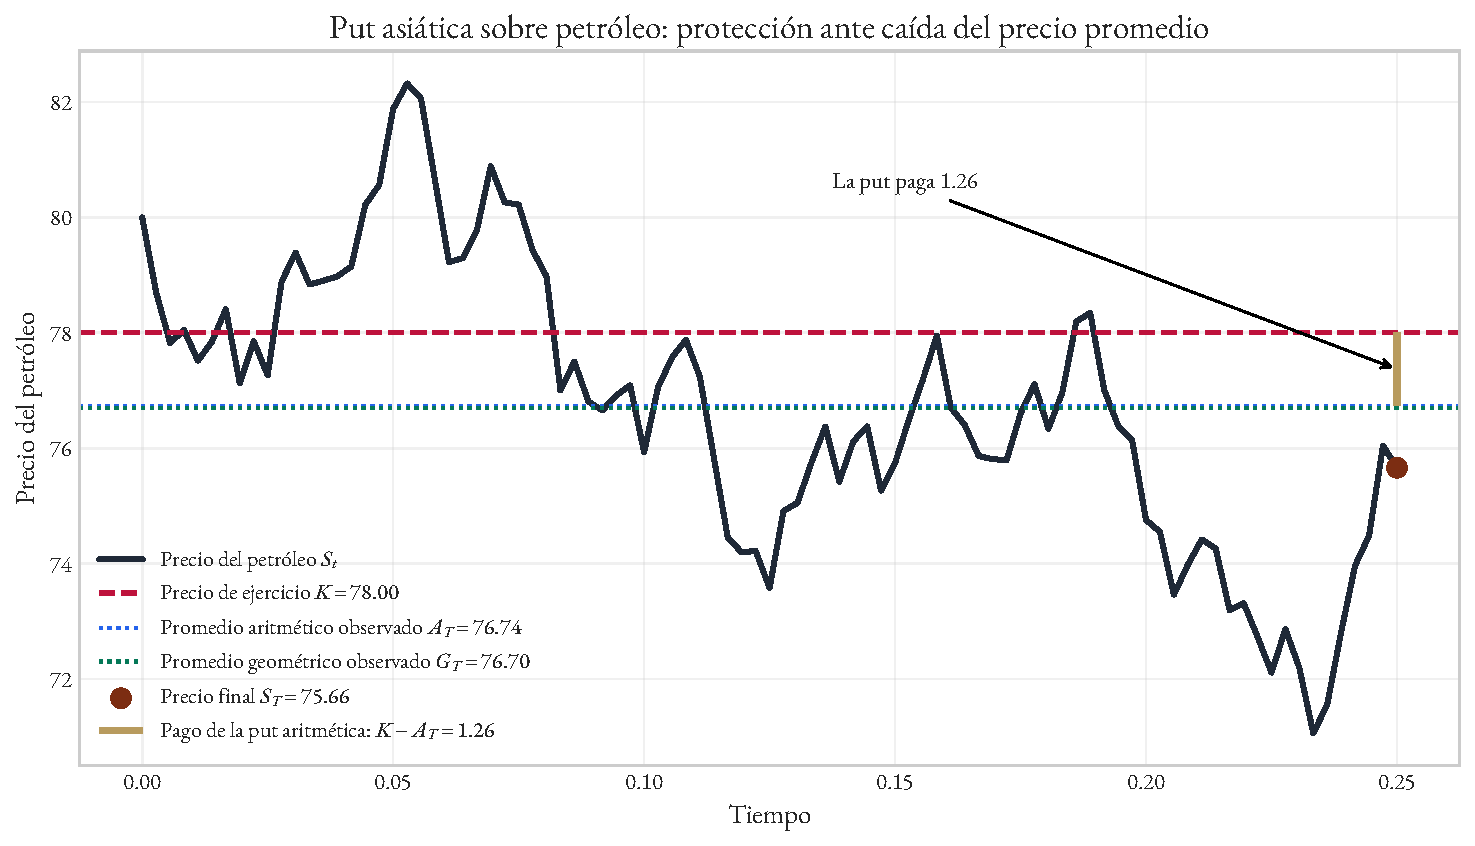
\includegraphics[width=0.70\linewidth]{asian_put_oil_path.pdf}
\caption{Ejemplo de una put asiática sobre petróleo. Se muestran el precio de ejercicio \(K\), el promedio aritmético \(A_T\), el promedio geométrico \(G_T\) y el precio final \(S_T\). Fuente: elaboración propia.}
\label{fig:asian-put-oil-path}
\end{figure}

La dependencia respecto al promedio modifica el perfil de riesgo del derivado. Una put vanilla europea concentra toda la exposición en el precio terminal \(S_T\); en cambio, una put asiática distribuye la exposición sobre la trayectoria completa del subyacente. Por esta razón, los movimientos extremos ocurridos en una sola fecha tienen menor efecto sobre el pago final. En términos financieros, el promedio suaviza la variabilidad del subyacente que entra en la función de pago y, por ello, bajo condiciones comparables, una opción asiática suele tener una volatilidad efectiva menor y una prima inferior a la de una opción vanilla equivalente.


\section{Marco probabilístico de valuación}

Formalmente, el modelo se construye sobre un espacio de probabilidad filtrado
\begin{equation}
\left(\Omega,\mathcal{F},(\mathcal{F}_t)_{0\leq t\leq T},\Prob\right),
\end{equation}
donde \(\Omega\) es el espacio muestral, \(\mathcal{F}\) es una \(\sigma\)-álgebra de eventos, \(\Prob\) es la medida histórica, y \((\mathcal{F}_t)_{0\leq t\leq T}\) es una filtración que representa la información disponible en el mercado a través del tiempo. En particular,
\begin{equation}
\mathcal{F}_s\subseteq \mathcal{F}_t\subseteq \mathcal{F},
\qquad
0\leq s\leq t\leq T.
\end{equation}

El proceso de precios del subyacente se denota por
\begin{equation}
(S_t)_{0\leq t\leq T}.
\end{equation}
Donde este proceso es adaptado a su filtración; es decir, para cada \(t\), la variable aleatoria \(S_t\) es \(\mathcal{F}_t\)-medible. Esto significa que el precio del subyacente en el tiempo \(t\) es conocido con la información disponible hasta ese instante. Asimismo, el pago del derivado al vencimiento, denotado por \(H_T\), es una variable aleatoria \(\mathcal{F}_T\)-medible, pues depende de la información acumulada hasta \(T\).

La valuación se realiza bajo una medida neutral al riesgo, denotada por \(\Q\). Esta medida es una probabilidad definida sobre \((\Omega,\mathcal{F})\), equivalente a la medida física \(\Prob\), lo cual se escribe como
\begin{equation}
\Q\sim\Prob.
\end{equation}
La equivalencia \(\Q\sim\Prob\) significa que ambas medidas asignan probabilidad cero a los mismos eventos, aunque no necesariamente asignan la misma probabilidad a cada escenario. Bajo \(\Q\), los precios descontados de los activos son martingalas respecto de la filtración \((\mathcal{F}_t)\) en ausencia de arbitraje \citep{shreve2004}.

Por ejemplo, si \(B_t\) denota la cuenta bancaria libre de riesgo y la tasa libre de riesgo \(r\) es constante y continuamente capitalizada, entonces
\begin{equation}
B_t=e^{rt}.
\end{equation}
En el caso más simple, sin dividendos ni costos de acarreo, el precio descontado del subyacente se define como
\begin{equation}
\widetilde S_t
:=
\frac{S_t}{B_t}
=
e^{-rt}S_t.
\end{equation}
La condición martingala bajo \(\Q\) exige que
\begin{equation}
\E^\Q\!\left[\widetilde S_T\mid\mathcal{F}_t\right]
=
\widetilde S_t,
\qquad
0\leq t\leq T.
\end{equation}
De forma equivalente,
\begin{equation}
S_t
=
e^{-r(T-t)}
\E^\Q\!\left[S_T\mid\mathcal{F}_t\right].
\end{equation}
Esta igualdad expresa que, bajo la medida neutral al riesgo, el precio actual del activo coincide con el valor presente de su valor futuro esperado. Por tanto, \(\Q\) no elimina la incertidumbre del mercado; modifica las probabilidades de los escenarios para que el crecimiento esperado descontado sea consistente con ausencia de arbitraje.

En el modelo generalizado de Black--Scholes utilizado para las opciones asiáticas, se permite que el subyacente tenga un costo de acarreo constante \(b\). Bajo la medida neutral al riesgo, se supone entonces que \(S_t\) sigue un movimiento geométrico browniano de la forma
\begin{equation}
\frac{\dd S_t}{S_t}
=
b\,\dd t+\sigma\,\dd W_t^\Q,
\end{equation}
donde \(\sigma>0\) es la volatilidad anual del subyacente y \(W_t^\Q\) es un movimiento browniano bajo \(\Q\). De manera equivalente,
\begin{equation}
\dd S_t
=
bS_t\,\dd t+\sigma S_t\,\dd W_t^\Q.
\end{equation}
La solución explícita de esta ecuación diferencial estocástica es
\begin{equation}
S_t
=
S_0
\exp\left[
\left(b-\frac{1}{2}\sigma^2\right)t+\sigma W_t^\Q
\right],
\end{equation}

donde \(b\) determina la deriva neutral al riesgo del subyacente, mientras que \(r\) determina el descuento de los pagos futuros. Por ello, las fórmulas de valuación contienen simultáneamente el factor de descuento \(e^{-rT}\) y el factor de crecimiento ajustado \(e^{(b-r)T}\).

Por ausencia de arbitraje, si \(H_T\) es el pago de un derivado al vencimiento, su precio en \(t=0\) se obtiene como
\begin{equation}
V_0
=
e^{-rT}\E^\Q[H_T],
\end{equation}
siempre que el pago sea replicable dentro del mercado considerado, es decir, que exista una estrategia de inversión en activos disponibles que genere el mismo pago \(H_T\) al vencimiento.

La dificultad sobre la valuación depende de la forma específica de este promedio. Si \(\bar S_T=G_T\), el logaritmo del promedio geométrico es normal y existe una fórmula cerrada. Si \(\bar S_T=A_T\), el promedio aritmético es una integral de variables lognormales correlacionadas y no tiene una distribución lognormal exacta; por ello se utiliza la aproximación por momentos de Turnbull--Wakeman.

\section{Caso de estudio}

El caso de estudio consiste en valuar una opción put asiática escrita sobre un activo subyacente con precio inicial \(S_0=80\), precio de ejercicio \(K=85\) y plazo de vencimiento de tres meses. Se supone una tasa libre de riesgo anual de \(r=5\%\), un costo de acarreo anual de \(b=8\%\) y una volatilidad anual de \(\sigma=20\%\). En unidades anuales, el plazo es \(T=0.25\). Por tanto, los parámetros del modelo son
\begin{equation}
S_0=80,
\qquad
K=85,
\qquad
r=0.05,
\qquad
b=0.08,
\qquad
\sigma=0.20,
\qquad
T=0.25.
\end{equation}

Primero se obtiene la prima de la put asiática con promedio geométrico. Después, usando la misma información de mercado, se calcula la prima de la put asiática con promedio aritmético mediante una aproximación por momentos. Finalmente, ambas primas se comparan con la prima de una put europea vanilla valuada bajo el modelo generalizado de Black--Scholes con costo de acarreo.

El propósito de la comparación es analizar la relación de orden entre las primas
\begin{equation}
P_{\mathrm{arit}},
\qquad
P_{\mathrm{geom}},
\qquad
P_{\mathrm{vanilla}},
\end{equation}
donde \(P_{\mathrm{arit}}\) corresponde a la put asiática aritmética, \(P_{\mathrm{geom}}\) a la put asiática geométrica y \(P_{\mathrm{vanilla}}\) a la put vanilla europea. En particular, se verifica si los resultados numéricos satisfacen
\begin{equation}
P_{\mathrm{arit}}
<
P_{\mathrm{geom}}
<
P_{\mathrm{vanilla}}.
\end{equation}

\section{Put asiática con promedio geométrico}

El promedio geométrico continuo es
\begin{equation}
G_T=\exp\left(\frac{1}{T}\int_0^T\ln S_u\dd u\right).
\end{equation}

Como \(\ln S_u\) es gaussiano y la integral temporal es una transformación lineal, \(\ln G_T\) también es gaussiano. Esto permite escribir una fórmula tipo Black--Scholes con parámetros ajustados, siguiendo la valuación de opciones asiáticas de promedio geométrico de \citet{kemna1990}:
\begin{equation}
\sigma_G=\frac{\sigma}{\sqrt{3}},
\qquad
b_G=\frac{1}{2}\left(b-\frac{\sigma^2}{6}\right).
\end{equation}

Los umbrales normales son
\begin{equation}
d_1^G=\frac{\ln(S_0/K)+(b_G+\frac{1}{2}\sigma_G^2)T}{\sigma_G\sqrt{T}},
\qquad
 d_2^G=d_1^G-\sigma_G\sqrt{T}.
\end{equation}

La prima de la put geométrica está dada por
\begin{equation}
P_G=Ke^{-rT}\PhiN(-d_2^G)-S_0e^{(b_G-r)T}\PhiN(-d_1^G).
\end{equation}

Con los parámetros considerados:
\[
\sigma_G=11.5470\%,
\qquad
b_G=3.6667\%,
\qquad
\ln(S_0/K)=-0.060625,
\]
\[
d_1^G=-0.862410,
\qquad
 d_2^G=-0.920145,
\qquad
\PhiN(-d_1^G)=0.805769,
\qquad
\PhiN(-d_2^G)=0.821252.
\]

La prima de la put asiática con promedio geométrico es
\resultbox{
\[
P_G=4.6922.
\]
}

\section{Put asiática con promedio aritmético}

El promedio aritmético continuo es
\begin{equation}
A_T=\frac{1}{T}\int_0^T S_u\dd u.
\end{equation}

A diferencia de \(G_T\), el promedio \(A_T\) no es lognormal de manera exacta. La aproximación de \citet{turnbull1991}, también presentada por \citet{hull2018}, consiste en construir una variable lognormal equivalente que iguale los dos primeros momentos del promedio aritmético:
\begin{equation}
\E[A_T]=M_1,
\qquad
\E[A_T^2]=M_2.
\end{equation}

Para costo de acarreo constante \(b\neq 0\), el primer momento es
\begin{equation}
M_1=S_0\frac{e^{bT}-1}{bT}.
\end{equation}

El segundo momento usado en la versión Hull/Turnbull--Wakeman es
\begin{equation}
M_2=\frac{2S_0^2}{T^2}
\left[
\frac{e^{(2b+\sigma^2)T}-1}{(b+\sigma^2)(2b+\sigma^2)}
-
\frac{e^{bT}-1}{b(b+\sigma^2)}
\right].
\end{equation}

La varianza lognormal efectiva se define como
\begin{equation}
\sigma_A^2=\frac{1}{T}\ln\left(\frac{M_2}{M_1^2}\right),
\qquad
\sigma_A=\sqrt{\sigma_A^2}.
\end{equation}

Los parámetros normales de la aproximación son
\begin{equation}
d_1^A=\frac{\ln(M_1/K)+\frac{1}{2}\sigma_A^2T}{\sigma_A\sqrt{T}},
\qquad
 d_2^A=d_1^A-\sigma_A\sqrt{T}.
\end{equation}

La prima aproximada de la put aritmética está dada por
\begin{equation}
P_A\approx e^{-rT}\left[K\PhiN(-d_2^A)-M_1\PhiN(-d_1^A)\right].
\end{equation}

Con los parámetros considerados:
\[
M_1=80.805360,
\qquad
M_2=6551.435171,
\qquad
\sigma_A^2=0.013411,
\qquad
\sigma_A=0.115807,
\]
\[
d_1^A=-0.845054,
\qquad
 d_2^A=-0.902957,
\qquad
\PhiN(-d_1^A)=0.800960,
\qquad
\PhiN(-d_2^A)=0.816726.
\]

La prima aproximada de la put asiática con promedio aritmético es
\resultbox{
\[
P_A=4.6415.
\]}

\section{Put vanilla con costo de acarreo}

Para la comparación, se valúa una put europea vanilla con los mismos datos \(S_0,K,r,b,\sigma,T\). Los parámetros Black--Scholes con costo de acarreo se obtienen de la extensión estándar del modelo lognormal de \citet{black1973}, como se presenta en \citet{hull2018}:
\begin{equation}
d_1^V=\frac{\ln(S_0/K)+(b+\frac{1}{2}\sigma^2)T}{\sigma\sqrt{T}},
\qquad
 d_2^V=d_1^V-\sigma\sqrt{T}.
\end{equation}

La prima de la put vanilla está dada por
\begin{equation}
P_V=Ke^{-rT}\PhiN(-d_2^V)-S_0e^{(b-r)T}\PhiN(-d_1^V).
\end{equation}

Con los parámetros considerados:
\[
d_1^V=-0.356246,
\qquad
 d_2^V=-0.456246,
\qquad
\PhiN(-d_1^V)=0.639172,
\qquad
\PhiN(-d_2^V)=0.675894.
\]

Por tanto, el precio de una put vanilla con costo de acarreo es
\resultbox{
\[
P_V=5.2186.
\]
}

\section{Comparación y relación de orden}

Las tres primas reflejan cuánta exposición conserva cada instrumento frente a movimientos adversos del subyacente. La put vanilla depende directamente del precio terminal \(S_T\). Por tanto, si al vencimiento el subyacente termina muy por debajo del precio de ejercicio, todo ese movimiento negativo entra directamente en el pago, lo que genera una compensación mayor, haciendo que la prima de la put vanilla sea más alta.

En cambio, una opción asiática no depende sólo del precio final, sino de un promedio de precios observados durante la vida del contrato. Ese promedio suaviza la trayectoria, una caída fuerte al final puede quedar compensada por precios anteriores más altos. Por esta razón, la volatilidad del promedio es menor que la volatilidad del precio final, lo que reduce el valor esperado del pago de la put asiática y, por ende, su prima. Por tanto, se espera que las primas de las puts asiáticas \(P_A\) y \(P_G\) sean menores que la prima de la put vanilla \(P_V\).

Entre las dos opciones asiáticas, la put geométrica resulta ligeramente más cara que la put aritmética porque el promedio geométrico es menor que el promedio aritmético por la desigualdad aritmético--geométrica, \textit{que se demuestra a partir de \( (x-y)^2 \geq 0 \)}. Como una put paga más cuando el precio que entra en el pago es menor, usar el promedio geométrico genera una base más favorable para el comprador de la put. En consecuencia, se espera que la put geométrica tenga una prima mayor que la put aritmética.

Esta intuición puede formalizarse mediante mediante definir a \(A_T\) y \(G_T\) el promedio aritmético y el promedio geométrico del subyacente durante la vida de la opción. Como los precios del subyacente son positivos, se cumple, trayectoria por trayectoria (es decir, para cada realización de la trayectoria del subyacente),
\begin{equation}
A_T\geq G_T.
\end{equation}
Por otro lado, la función de pago de una put es decreciente respecto al argumento promedio. Es decir, si \(x_1\geq x_2\), entonces
\[
\max\{K-x_1, 0\}\leq \max\{K-x_2, 0\}.
\]
Al aplicar esta propiedad a \(A_T\) y \(G_T\), se obtiene
\begin{equation}
\max\{K-A_T, 0\}\leq \max\{K-G_T, 0\}.
\end{equation}
Por lo tanto, al descontar y tomar esperanza bajo la medida neutral al riesgo,
\begin{equation}
P_A
=
e^{-rT}\mathbb{E}^{\mathbb{Q}}\!\left[\max\{K-A_T, 0\}\right]
\leq
e^{-rT}\mathbb{E}^{\mathbb{Q}}\!\left[\max\{K-G_T, 0\}\right]
=
P_G.
\end{equation}

La comparación contra la put vanilla no proviene de una desigualdad trayectoria por trayectoria tan directa, porque \(S_T\) puede estar por encima o por debajo del promedio de la trayectoria. Sin embargo, para los parámetros del ejercicio, el efecto de suavizamiento de las opciones asiáticas reduce su valor frente a la put vanilla. Numéricamente, se obtuvo
\[
P_A=4.6415,
\qquad
P_G=4.6922,
\qquad
P_V=5.2186.
\]
Por tanto, se verifica la relación de orden
\begin{equation}
P_A<P_G<P_V.
\end{equation}

En conclusión, la relación de orden \(P_A<P_G<P_V.\) sí se cumple para los parámetros del caso de estudio:

\resultbox{
\[
P_{\mathrm{arit}}=4.6415
<
P_{\mathrm{geom}}=4.6922
<
P_{\mathrm{vanilla}}=5.2186.
\]
}

\section{Conclusión}

El caso de estudio muestra que las opciones asiáticas son relevantes por la forma en que representan riesgos económicos reales. En muchos mercados, especialmente en materias primas y energía, las decisiones financieras no dependen únicamente del precio observado al vencimiento, sino del comportamiento promedio del activo durante un periodo. Por eso, una opción asiática puede ser una cobertura más cercana al riesgo operativo de una empresa que una opción vanilla.

El promedio geométrico permite una fórmula cerrada porque el logaritmo del promedio es normal bajo movimiento geométrico browniano \citep{kemna1990}. En cambio, el promedio aritmético requiere una aproximación porque una integral de lognormales correlacionadas no es lognormal exacta. La aproximación Turnbull--Wakeman/Hull resuelve esta dificultad práctica mediante igualación de momentos \citep{turnbull1991,hull2018}. 

Con los parámetros considerados se obtuvo la relación
\[
P_{\mathrm{arit}}=4.6415<P_{\mathrm{geom}}=4.6922<P_{\mathrm{vanilla}}=5.2186.
\]
Esta relación confirma la intuición de que la opción vanilla es más cara porque conserva toda la exposición al precio terminal; las asiáticas, en cambio, suavizan la trayectoria mediante un promedio y reducen la volatilidad efectiva del activo que entra en el pago. Además, entre las dos asiáticas, la put geométrica resulta más cara que la aritmética porque el promedio geométrico no excede al promedio aritmético, lo que aumenta el pago esperado de una put.

El ejemplo de Pemex ayuda a interpretar el resultado de como una empresa expuesta a cambios en el precio del subyacente puede usar derivados para transformar su perfil de riesgo, y aunque el resultado contable de esos instrumentos puede ser positivo o negativo dependiendo de la evolución del mercado, la finalidad de la cobertura no es maximizar el resultado del derivado, sino reducir la incertidumbre de los flujos de efectivo y hacer más estable la planeación financiera.

La valuación de estos instrumentos permite asignar una prima consistente con el riesgo modelado, pero la elección del derivado depende del riesgo que se desea cubrir. Si el riesgo económico está asociado a un precio final, una opción vanilla puede ser adecuada; si está asociado a un precio promedio durante el periodo, una opción asiática puede representar mejor la exposición real. Esta es precisamente la importancia de los derivados exóticos: adaptar el contrato financiero a la forma concreta en que aparece el riesgo en la operación de una empresa.

\newpage
\nocite{curso2026}
\bibliographystyle{apalike}
\bibliography{biblo}

\end{document}
